\documentclass[11pt, twoside, a4paper]{article}
\usepackage[italian]{babel}
\usepackage[utf8]{inputenc}
\usepackage{amsmath}
\usepackage{fullpage}
\usepackage{graphicx}
\usepackage{booktabs}
\usepackage{wrapfig}
\usepackage{multirow}
\usepackage{sidecap}
\usepackage{siunitx}
\usepackage[font=small]{caption}
\usepackage[bookmarks, bookmarksopen, hidelinks]{hyperref}

\begin{document}

\begin{titlepage}
\begin{center}

	\hrule \vspace{0.5cm}
     	\textsc{\LARGE STUDIO DEL PERIODO DI UN PENDOLO SEMPLICE.\\}
     	\vspace{0.4cm}
     	\textsc{\LARGE MISURAZIONE DELL'ACCELERAZIONE DI GRAVITA'.}
	\vspace{0.5cm} \hrule \vspace{2cm}

      	{\large Francesco Pasa, Davide Bazzanella, Andrea Miani\\
		Gruppo A11}\\
	\vspace{0.5cm}
      	{\large 8 Aprile 2013 - 22 Aprile 2013}
	\vfill

	
\includegraphics[width=4cm]{unitn_logo.png}\\
	\vspace{1cm}
        \textsc{\Large Università degli studi di Trento}
	\vfill

	{\begin{abstract}
        Studio della dipendenza del periodo di oscillazione dalla massa e dalla lunghezza del pendolo.
        Calcolo dell'accelerazione di gravità a partire dai dati di periodo e lunghezza del pendolo.
	 \end{abstract}}
\end{center}
\end{titlepage}

\newpage
\vspace*{\fill}
\begin{center}
	\tableofcontents
\end{center}
\vspace*{\fill}
\newpage
\section{Introduzione}


In questo esperimento studieremo in modo quantitativo quali relazioni sussistano tra il periodo di oscillazione di un pendolo $\mathcal{T}$, la massa applicatavi $m$ e la lunghezza del filo stesso $l$.\\
Queste relazioni, nel caso di piccole oscillazioni, furono studiate e formalizzate per la prima volta da Galileo Galilei (Pisa, 15 febbraio 1564 – Arcetri, 8 gennaio 1642) e si possono riassumere come segue:

\begin{equation}
    \label{eq:periodo_pendolo}
	\mathcal{T} \,=\, 2\pi\sqrt{\frac{l}{g}}
\end{equation}
%
dove $g$ rappresente l'accelerazione di gravità (locale).\\
Quindi in questo esperimento ci proponiamo di verificare che il periodo di oscillazione di un pendolo,
sfruttando il modello di pendolo semplice, sia legato alla lunghezza del filo da una proporzionalità del tipo $\sqrt{\ell}$,
e che non abbia dipendenza dalla massa.
Inoltre coi dati che andremo a raccogliere abbiamo intenzione di ricavare un valore sperimentale dell'accelerazione di gravità.


\section{Dipendenza del periodo del pendolo dalla massa}
%\input{massa.tex}
%bla bla bla - introduzione alla massa
	\subsection{Apparato Sperimentale}
	---

	\subsection{Procedura di misura}
	L'acquisizione dei dati sperimentali è avvenuta nel seguente modo:
\begin{itemize}
	\item{abbiamo costruito il pendolo applicando al filo da pesca, di massa trascurabile, una delle tre masse simili tra loro, e successivamente abbiamo appeso l'apparato al supporto;}
	\item{abbiamo rilevato il periodo di oscillazione del pendolo cronometrando un ciclo di 5 oscillazioni per quindici volte, cinque per ogni componente del gruppo, in modo da ridurre l'errore sistematico sulla misura dovuto ad una differente prontezza di riflessi dei singoli operatori;}
	\item{abbiamo prestato attenzione che l'ampiezza delle oscillazioni fosse contenuta entro 10 gradi grazie al disegno dell'angolo massimo su un foglio di carta. Abbiamo inoltre cercato di fare in modo che le oscillazioni fossero contenute in un piano e non compissero un moto elittico.}
\end{itemize}

	\subsection{Analisi dati}
	\subsubsection{Considerazioni iniziali}
In questa prima parte della relazione vogliamo verificare che il periodo di oscillazione del pendolo, a parità di lunghezza del filo, non dipende dalla massa applicatavi.
Per fare questo abbiamo cronometrato il periodo di ocillazione del pendolo per tutte e quattro le masse a nostra disposizone.\\
Poichè abbiamo utilizzato l'approssimazione di pendolo semplice, nel quale la massa si considera totalmente applicata in un unico punto, è importante sottolineare che, quando è stata presa la misura del periodo relativo alla massa più piccola, abbiamo dovuto regolare la lunghezza del filo in modo che il baricentro della massa risultasse essere alla stessa distanza dal morsetto, a cui è applicato il filo, rispetto alle masse precedenti.\\
Ricordiamo inoltre che per ottenere la lunghezza complessiva del filo si è seguita la seguente procedura: la lunghezza complessiva del filo è data da:

\begin{equation}
	\l_{tot} \,=\, l_{filo} + \frac{h}{2} - l_{morsetto}
\end{equation}
%
dove $l _{filo}$ è la lunghezza del filo misurata dall'estremo superiore del morsetto fino al punto di applicazione sulla massa, $l_{morsetto}$ è l'altezza del morsetto e $\frac{h}{2}$ è l'altezza che rappresenta il baricentro della massa.\\
Pertanto l'errore sulla misura della lunghezza del filo sarà dato dalla propagazione dell'errore per la somma di misure indipendenti, ovvero:

\begin{equation*}
	\delta l_{tot} \,=\, \sqrt{(\delta l_{filo})^2 + (\delta \frac{h}{2})^2 + (\delta l_{morsetto})^2}
\end{equation*}
%
ricordando che le inceretzze relative alle varie misure sono le incertezze tipo, ovvero:

\begin{equation*}
	\text{inceretzza tipo su l} \,=\, \frac{\Delta l}{\sqrt{12}}
\end{equation*}
%
Mentre le masse sono affette da un incertezza tipo pertanto ogni massa avrà la seguente incertezza:

\begin{equation*}
	\delta m \,=\, \frac{\Delta m}{\sqrt{12}} \,=\, 0.03 \,\, g
\end{equation*}

\subsubsection{Dati}
Le masse che abbiamo applicato al filo da pesca sono quelle esposte nella \ref{masse} mentre nella \ref{periodi} sono elencati tutti i periodi che abbiamo rilevato per ciascuna massa.\\

Procediamo ora calcolando la media dei periodi per le quattro masse da noi considerate. Ricordiamo che:

\begin{equation*}
	\mathcal{T} \,=\, m[t]^* \,=\, \frac{\sum_{i}^{N} t_i}{N}
\end{equation*}
%
e che l'errore sulla media dei periodi risulta essere:

\begin{equation*}
	\delta \mathcal{T} \,=\, \frac{1}{\sqrt{N}} \, \tilde\sigma[\mathcal{T}] \quad \text{dove} \quad \tilde\sigma[\mathcal{T}] \,=\, \frac{1}{N-1} \sum_{i}^{N} (t_i - m[t]^*)^2
\end{equation*}
%
pertanto otteniamo:

%Dal momento che lo scopo di questa prima analisi è quella di verificare se sussiste una dipendenza tra periodo di oscillazione del pendolo e massa applicatavi, procediamo con l'analizzare il \ref{grafico masse vs periodi}.\\
%Come si può notare, non siamo in grado di individuare le rette di massima e minima pendenza in quanto le barre di errore risultano essere troppo piccole, anche rispetto alla rappresentazione puntiforme del dato nel grafico. Ciononostante osserviamo che la retta sembra essere una retta costante e pertanto possiamo ipotizzare che il valore del suo coefficiente angolare dovrebbe essere zero.\\
%Questa ipotesi non semra essere così errata in quanto è stato provato ripetutamente che la legge del pendolo applicata ad un modello di pendolo semplice per piccole oscillazioni mostra che il periodo di ocsillazione non dipende dalla massa applicata al filo. 


%Nonostante questo possiamo provare a calcolare il coefficiente angolare della retta per avere una minima %idea del valore che esso assume. Pertantio il coefficiente angolare della retta sarà ricavato come segue:

%\begin{equation*}
%	\text{k} \,=\, \frac{t_4 - t_1}{m_4 - m_1} 
%\end{equation*}
%
%e l'errore che affligge questa misura si puòricavare nel seguente modo:

%\begin{equation}
%	\frac{(\delta k)^2}{k^2} \,=\, \frac{\delta}{•}
%\end{equation}
		\subsubsection{Medie pesate}
		---

		\subsubsection{Test del chi quadro}
		\label{m_chi_pesata}

Dopo aver calcolato la media pesata delle misure $\mathcal{T}_i\,$ sfruttiamo il test del chi quadro per verificare se
è ammissibile che il periodo del pendolo non dipenda dalla massa. Tramite la procedura della media pesata (che è una regressione
a tutti gli effetti) abbiamo ottenuto
una retta orizzontale il cui valore costante è $\mathcal{T}_w$. Se il test del chi quadro risulterà positivo questo indicherà
che i periodi al variare della massa sono compatibili con un andamento costante, e quindi che il periodo non dipende dalla massa.

%Per questo motivo defiano la seguente funzione $f$

%\begin{equation}
%	f \,:=\, A + B m 
%\end{equation}
%
%dove B rappresenta il coefficiente angolare della retta, che assumiamo nullo, $m$ la massa applicata al pendolo e A una costante che nel nostro caso particolare è il valore della media pesata dei periodi ($\mathcal{T}$).\\
%Pertanto ora procediamo nell'eseguire il test del chi quadro per accertarci se il risultato da noi trovato sia accettabile o meno.
Calcoliamo quindi il chi quadro osservato:

\begin{equation*}
	\chi_{oss}^2 \,=\, \frac{\sum_{i=0}^{\mathcal{N}} (\mathcal{T}_i - \mathcal{T}_w)^2}{(\delta \mathcal{T}_i)^2} \,=\, 1.66
\end{equation*}
%
%è importante sottolineare che il $\delta \mathcal{T}$ non è altro che $\delta \mathcal{T}_i$ in quanto $B = 0$ per ipotesi.
dove $\mathcal{T}_i$ rappresentano le quattro misure medie del periodo relative alle quattro massa considerate e $\mathcal{T}_w$ rappresenta il valore della media pesata trovato precedentemente. $\mathcal{N} = 4$ è il numero di masse. In figura \ref{fig:masse_periodi} sono
riportati i punti sperimentali con le barre d'errore e la media pesata, ed è possibile calcolare approssimativamente il chi quadro. \\

I gradi di libertà del nostro sistema sono 3 e che vogliamo una probabilità del $5\%$ che i dati da noi raccolti non siano in accordo con le ipotesi fatte finora, quindi abbiamo posto la probabilità di falso allarme al $5\%$, otteniamo che l'intervallo di accettazione del $\chi_{oss}^2$ va da 0 a 7.82.\\
Siccome il $\chi_{oss}^2$ ha valore di 1.66, esso ricade all'interno dell'intervallo di accettazione. Quindi possiamo dire che il periodi rilevati
al variare della massa sono compatibili con un andamento costante. I dati sperimentali indicano dunque che
il periodo del pendolo non dipende dalla massa. Ovvero noi sappiamo che mediamente una volta su venti può accadere che il dato sperimentale raccolto risulti essere in contraddizione con le ipotesi fatte, in particolare con quella che nega una dipendenza del periodo dalla massa.\\
Abbiamo ricavato i valori degli estremi di accettazione del chi quadro grazie ad un programma presente sul sito internet stattrek.com\footnote{
\url{http://stattrek.com} è un sito dedicato alla statistica. La pagina che abbiamo utilizzato per calcolare la distribuzione del chi quadro
è raggiungibile all'indirizzo \url{http://stattrek.com/online-calculator/chi-square.aspx}.}.

		\subsubsection{Regressione lineare}
		Come prima operazione defiano la seguente funzione $f$

\begin{equation}
	f \,:=\, A + B m 
\end{equation}
%
dove B rappresenta il coefficiente angolare della retta, che assumiamo nullo, $m$ la massa applicata al pendolo e A una costante che nel nostro caso particolare è il valore della media pesata dei periodi ($\mathcal{T}$).\\

\begin{SCfigure}
    \centering
    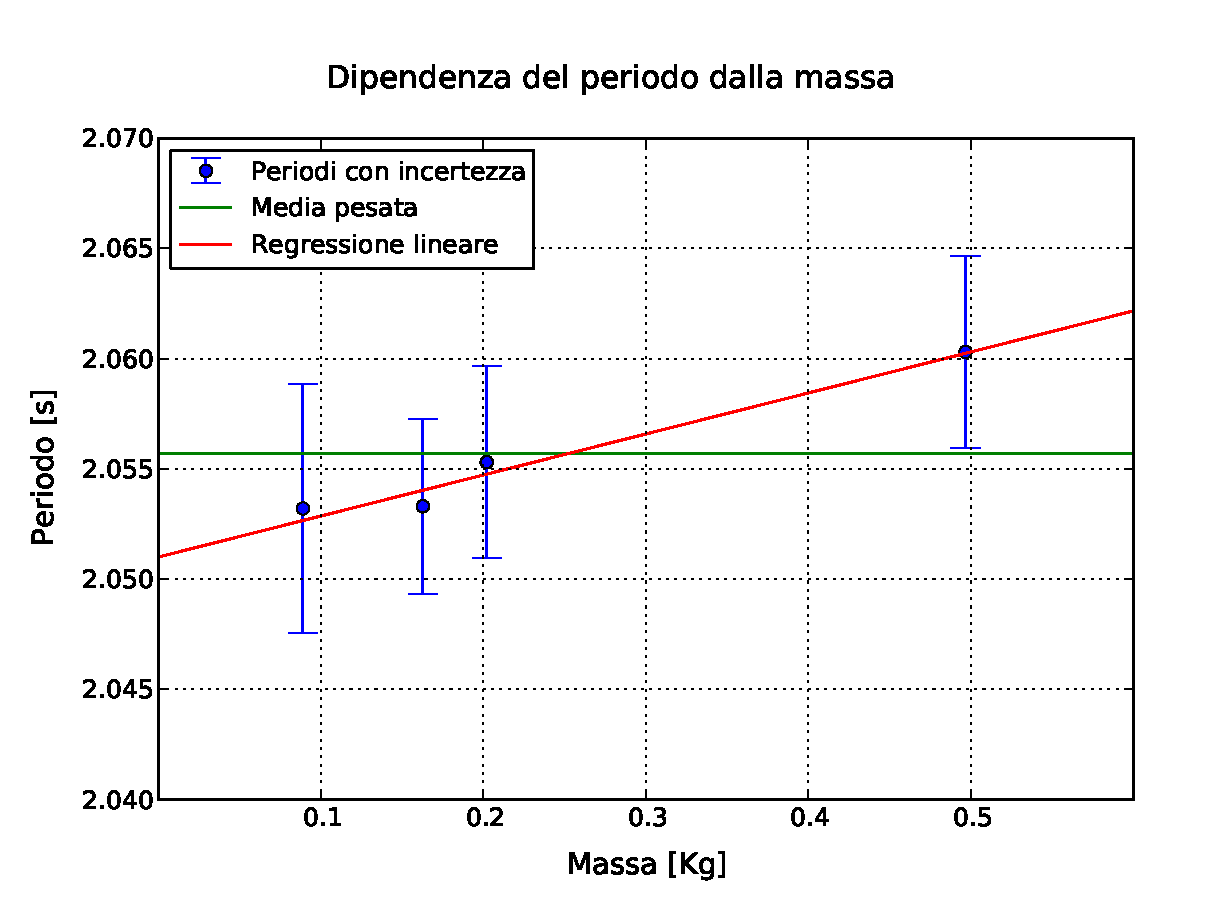
\includegraphics[width=110mm]{immagini/masse.pdf}
    \caption{Il seguente grafico rappresenta sull'asse delle ordinate le medie dei periodi relativi ad ogni
        singola massa, mentre sull'asse delle ascisse sono riportate le masse utilizzate. L'incertezza sul periodo
        è differente da misura a misure, mentre quella reativa alla massa è uguale per tutte, ed in particolare è
        l'incertezza tipo. La retta orizzontale verde rappresenta il valore (costante) della media pesata delle medie
        dei periodi ($\mathcal{T}$), mentre in rosso è rappresentata la retta derivante dalla regressione lineare,
        ovvero la funzione $\mathcal{T} = A + B\,m$.}
    \label{fig: periodo vs masse}
\end{SCfigure}

Finora abbiamo assunta veritiera l'ipotesi che il periodo di oscillazione del pendolo non dipende linearmente dalla massa applicata. Ciononostante ora vogliamo controllare se effettivamente sia così e quindi abbiamo deciso di fare una regressione lineare sulla funzine $f$ in modo da dare una stima ai parametri A e B e verificare che A risulti compatibile con il periodo del pendolo $\mathcal{T}$ trovato grazie alla media pesata e che il valore di B sia compatibie con lo 0 teorico.\\

Procediamo operativamente in questo modo per eseguire la regressione lieare:

\begin{itemize}
	\item{Grazie al grafico sopra riportato \ref{fig: periodo vs masse} diamo una stima preliminate dei due parametri A e B, in questo modo: al parametro A è stato associato il vlore del periodo ($\mathcal{T}$) trovato grazie alla media pesata, mentre per avere una stima del parametro B abbiamo deciso di calcolare il coefficiente angolare della retta che intercetta i dati, ovvero:
			\begin{equation*}
				A \,=\, \mathcal{T}; \quad \quad B \,=\, \frac{\mathcal{T}_4 - \mathcal{T}_1}{m_4 - m_1} \,=\, 0.017165
			\end{equation*}
			%
			}
	\item{La funzione da minimizzare che misura la discrepanza è:
			\begin{equation}
                \sum_{i=1}^{N} \frac{(\mathcal{T}_i - A - B m_i)}{(\delta \mathcal{T}_{tot})^2}	
                \label{eq:min_quad}
			\end{equation}
			%
            dove $\delta \mathcal{T}_{tot}$ è l'incertezza totale sulle misure del periodo, ottenuta sommando l'incertezza $\delta \mathcal{T}_i$ e l'errore trasferito dal peso, che risulta essere però trascurabile rispetto all'incertezza sul periodo poichè $\delta \mathcal{T}_i$ risulta essere dell'ordine di grandezza di $10^{-3}$ mentre l'incertezza trasferita dalla massa è dell'ordine di $10^{-6}$, e quindi quest'ultima risulta essere trascurabile rispetto all'incertezza sul periodo;}
	\item{Quindi per quanto studiato in classe abbiamo che:

			\begin{equation*}
				A \,=\, \frac{(\sum_i w_i m_i^2)(\sum_i w_i \mathcal{T}_i) - (\sum_i w_i m_i)(\sum_i w_i m_i \mathcal{T}_i)}{\Delta} \,=\, 2.0510 \,\, s
			\end{equation*}
			%
			\begin{equation*}
				B \,=\, \frac{(\sum_i w_i)(\sum_i w_i m_i \mathcal{T}_i) - (\sum_i w_i \mathcal{T}_i)(\sum_i w_i m_i)}{\Delta} \,=\, 0.01862
			\end{equation*}
			%
			dove:
			\begin{equation*}
				\Delta \,=\, (\sum_i w_i)(\sum_i w_i m_i^2) - (\sum_i w_i m_i)^2 \,\,\,\,\,\,\, e \,\,\,\,\,\,\,
				w_i \,=\, \frac{1}{(\delta \mathcal{T}_i)^2}
			\end{equation*}}
	\item{Di conseguenza abbiamo che le incertezze relative su A e B sono:

			\begin{equation*}
				(\delta A)^2 \,=\, \frac{\sum_i w_i m_i^2}{\Delta}  \,\,\,\,\, e \,\,\,\,\,
				(\delta B)^2 \,=\, \frac{\sum_i w_i}{\Delta} 
			\end{equation*}}
	\end{itemize} 
	Quindi possiamo riassumere i risultati di questa procedura in questo modo:

	\begin{equation*}
		A \,\pm\, \delta A \,=\, (2.051 \,\, \pm \,\, 0.004) \,\,s \,\,\,\,\, e \,\,\,\,\,
		B \,\pm\, \delta B \,=\, (0.018602 \,\, \pm \,\, 0.014691) \,\,
	\end{equation*}
	%
Quindi non ci rimane altro che verificare se i due parametri così trovati risultano compatibili con quelli ipotizzati, ovvero A deve risultare essere compatibile con il periodo medio del pendolo calcolato grazie alla media pesata, mentre B deve risultare essere compatibile con lo 0 teorico. Pertanto posto a priori un fattore di copertura pari a tre ($k = 3$):

\begin{itemize}
	\item{calcoliamo la disrepanza (R) tra $\mathcal{T}$ ed A, ottenendo:
			\begin{equation*}
				R \,=\, \mathcal{T} - A \,=\, 0.005 \,s
			\end{equation*}
			%
			}
	\item{verificiamo ora se $R \leq k\,\sigma[R]$, dove:
			\begin{equation*}
				\sigma[R] \,=\, \sqrt{(\delta \mathcal{T})^2 + (\delta A)} \,=\, 0.004 \, s
			\end{equation*}
			%
			pertanto otteniamo che:
			\begin{equation*}
				R \leq k\,\sigma[R] \quad \text{in quanto} \quad 0.005 \, s \leq 0.013 \, s
			\end{equation*}
			%
			e quindi $\mathcal{T}$ risulta compatibile con A}
	\item{troviamo ora la discrepanza (R) tra $B$ ed il valore teorico 0, ottenendo:
			\begin{equation*}
				R \,=\, B - 0 \,=\, 0.0186
			\end{equation*}
			%
			}
	\item{controlliamo ora se $R \leq k\,\sigma[R]$, dove:
			\begin{equation*}
				\sigma[R] \,=\, \sqrt{(\delta A)^2} \,=\, 0.0147	
			\end{equation*}
			%
			pertanto otteniamo che:
			\begin{equation*}
				R \leq k\,\sigma[R] \quad \text{in quanto} \quad 0.0186 \leq 0.0441
			\end{equation*}
			%
			e quindi B risulta compatibile con lo 0 teorico}			
\end{itemize}
Quindi garzie a questa breve analisi abbiamo trovato che le ipotesi fatte inizialmente risultano essere corrette in quanto abbiamo verificato che il periodo del pendolo non dipende dalla massa applicata, restringendoci a considerare il nostro modello a quello di pendolo semplice e considerando le masse puntiformi.

%A =  2.0510
%B =  0.018602
%sigma_A =  0.0042932
%sigma_B =  0.014691
%chi2_fit =  0.057346

	\subsection{Conclusioni intermedie !-!-!-!-!-!-!-!-!-!-!-!-!-!-!}
	Quindi grazie a quanto illustrato finora abbiamo verificato che, data una lunghezza fissata, il periodo di oscillazione del pendolo non dipende dalla massa applicata ad esso. Inoltre possiamo dire che non c'è stata nemmeno un deformazione apprezzabile del filo utilizzato in quanto tutte le misure effettuate risultano compatibili con i valori ottenuti.

La non dipendenza del periodo dalla massa si può anche ricavare grazie ad un analisi dimensionale; ovvero: se supponiamo che il periodo del pendolo $\mathcal{T}$ possa dipendere dalla massa appesa $m$, dalla lunghezza del filo $\ell$ e dall'accelerazione di gravità $g$ mediante una relazione del tipo $\mathcal{T} \,\propto\, m^\alpha \, \ell^\beta \, g^\gamma$.\\
Studiando le dimensioni di $\mathcal{T}, \,\, m, \,\, \ell \,\,e\,\, g$ si ottiene che l'equazione dimensionale corretta è la seguente:

\begin{equation*}
	[T]^1 \,=\, [M]^\alpha[L]^{\beta+\gamma}[T]^-2\gamma 
\end{equation*}
%
che risulta essere soddisfatta per

\begin{equation*}
	\alpha \,=\, 0; \quad \gamma \,=\, -1/2; \quad \beta \,=\, -\gamma \,=\, 1/2 
\end{equation*}
%
da cui abbiamo che:

\begin{equation*}
	\mathcal{T} \,=\, \mathcal{C} \, \sqrt{\frac{\ell}{g}}
\end{equation*}
%
dove il parametro $\mathcal{C}$ è una costante il cui valore non si può determinare dal semplice calcolo dimensionale. Si nota che, poichè risulta essere necessario che $\alpha$ sia uguale a 0, allora anche dall'analisi dimensionale abbiamo ottenuto una conferma che effettivamente il periodo di oscillazione di un pendolo non dipende dalla massa applicata.

\newpage
\section{Dipendenza dalla linghezza}
	%Come già fatto nel caso, del tutto analogo, del
periodo di oscillazione di una molla, siamo andati a verificare la dipendenza
del periodo del pendolo al variare della lungezza del filo.

	%bla bla bla - introduzione alla lunghezza
	\subsection{Apparato Sperimentale}
	L'apparato sperimentale usato in questa seconda parte dell'esperimento è
identico a quello usto nella prima parte. In questo caso abbiamo usato una sola massa,
ovvero il cilindro di ottone più massiccio.

	\subsection{Procedura di misura}
	Abbiamo scelto 10 diverse lunghezze del filo, riportate in tabella \ref{tab:lunghezze_filo}.

\begin{table}
    \centering
    \begin{tabular}{c c c c c c c c c c}
        \multicolumn{10}{c}{\textbf{Lunghezze del filo [cm]}} \\
        \toprule
        105.7 & 95.3 & 85.3 & 75.3 & 65.3 & 55.3 & 45.3 & 35.3 & 25.3 & 15.3 \\
        \bottomrule
    \end{tabular}
    \caption{Lunghezze del filo scelte per testare la dipendenza del periodo
        del pendolo dalla lunghezza. Le dieci misure sono equispaziate ad intervalli di \SI{10}{\centi\metre}.}
    \label{tab:lunghezze_filo}
\end{table}

\begin{table}
    \centering
    \begin{tabular}{c c c c c c c c c c c}
        \multicolumn{11}{c}{\textbf{Lunghezze e periodi}} \\
        \toprule
        Lunghezza [m] & \multicolumn{10}{c}{Periodi [s]} \\
        \midrule
        1.057 & 2.086 & 2.068 & 2.052 & 2.040 & 2.054 & 2.062 & 2.098 & 2.048 & 2.058 & 2.048 \\
        0.953 & 1.932 & 1.942 & 1.948 & 1.928 & 1.954 & 1.946 & 1.954 & 1.958 & 1.944 & 1.968 \\
        0.853 & 1.844 & 1.860 & 1.864 & 1.864 & 1.862 & 1.860 & 1.854 & 1.854 & 1.858 & 1.840 \\
        0.753 & 1.732 & 1.726 & 1.720 & 1.742 & 1.754 & 1.742 & 1.740 & 1.744 & 1.748 & 1.746 \\
        0.653 & 1.604 & 1.626 & 1.614 & 1.610 & 1.598 & 1.620 & 1.600 & 1.614 & 1.614 & 1.596 \\
        0.553 & 1.448 & 1.494 & 1.498 & 1.472 & 1.454 & 1.472 & 1.480 & 1.488 & 1.488 & 1.472 \\
        0.453 & 1.348 & 1.336 & 1.326 & 1.348 & 1.330 & 1.336 & 1.332 & 1.340 & 1.346 & 1.308 \\
        0.353 & 1.182 & 1.196 & 1.190 & 1.188 & 1.198 & 1.176 & 1.182 & 1.160 & 1.204 & 1.194 \\
        0.253 & 1.002 & 1.018 & 0.996 & 1.012 & 1.018 & 1.024 & 0.998 & 0.998 & 0.994 & 1.022 \\
        0.153 & 0.762 & 0.774 & 0.790 & 0.794 & 0.790 & 0.768 & 0.770 & 0.768 & 0.794 & 0.772 \\
        \bottomrule
    \end{tabular}
\end{table}

	\subsection{Analisi dati}
	%\input{•}
		\subsubsection{Medie (errore)}
		\label{l_medie}

Innanzitutto vogliamo specificare le incertezze a cui sono soggetti i nostri dati.

Le lunghezze $\bar{l}_i$ del filo e la lunghezza del morsetto $l\ped{mors}$ sono state misurate con un metro a nastro di risoluzione
$\Delta l$ = 0.001 m. L'errore standard di risoluzione di queste misure vale quindi:

\begin{equation}
    \sigma(l) = \frac{\Delta l}{\sqrt{12}} = \SI{0.0003}{\metre}
\end{equation}

L'altezza $h$ del cilindro è stata misurata con un calibro ventesimale di risoluzione $\Delta l\ped{calibro} = 0.00005$ m
per cui l'errore tipo di risoluzione è:

\begin{equation}
    \sigma\ped{calibro}(l) = \frac{\Delta l\ped{calibro}}{\sqrt{12}} = \SI{0.00001}{\metre}
\end{equation}

Poichè abbiamo utilizzato il modello del pendolo semplice, siamo interessati a conoscere la distanza tra il punto
di sospensione ed il baricentro del cilindro. Il cilindro, la cui densità è stata considerata omogenea,
viene così approssimato ad un punto materiale posto nel suo centro. Vedremo in seguito come migliorare questa approssimazione.
Per ottenere la distanza tra punto di sospensione del filo e baricentro del cilindro si è usata la formula

\begin{equation}
	\l_i \,=\, \bar{l}_i \,-\, l\ped{mors} \,+\, \frac{h}{2}
    \label{eq:l_i}
\end{equation}

che è stata applicata ad ogni lunghezza del filo. I risultati dei calcoli sono riportati nella prima colonna
della tabella \ref{tab:l_dati}. L'incertezza sulla lunghezza trovata con la (\ref{eq:l_i}) si può ricavare mediante la propagazione
degli errori:

\begin{equation}
	\delta l_i = \sqrt{4\,\sigma(l)^2 + \left(\frac{\sigma\ped{calibro}(l)}{2}\right) ^2}
\end{equation}

\begin{SCtable}
    \centering
    \begin{tabular}{c c}
        \multicolumn{2}{c}{\textbf{Dati}} \\
        \toprule
        $l_i$ [m] & Periodo [s] \\
        \midrule
        1.0526 &  \\
        0.9486 &  \\
        0.8486 &  \\
        0.7486 &  \\
        0.6486 &  \\
        0.5486 &  \\
        0.4486 &  \\
        0.3486 &  \\
        0.2486 &  \\
        0.1486 &  \\
        \bottomrule
    \end{tabular}
    \caption{}
    \label{tab:l_dati}
\end{SCtable}

		\subsubsection{Test del chi quadro}
		Verifichiamo la bontà della regressione eseguita nel paragrafo precedente tramite il test del chi quadro.
Il valor atteso $\chi^2_{\text{teo}}$ del test è uguale al numero di gradi di libertà del sistema. Nel nostro caso
esso vale $\chi^2_{\text{teo}} = N - 2 = 8$ poiché dal fit sono stati calcolati 2 parametri. Poiché
il numero di gradi di libertà è basso, abbiamo deciso di adottare un intervallo di confidenza del tipo $[0, h]$,
dove $h$ è il valore critico del chi quadro. Scelta la probabilità di falso allarme del 5 \%, dalla distribuzione
del chi quadro si può calcolare $h = 15.5$. Quindi l'intervallo di confidenza è [0, 15.5]. 

Utilizzando i valori $A$ e $b$ trovati precedentemente, calcoliamo l'espressione

\begin{equation}
    \chi^2_{\text{oss}} = \sum_{i=1}^N \frac{(Y_i - A - bX_i)^2}{\delta Y_i^{\text{tot}}} = 29.4
\end{equation}
%
che è chiaramente al di fuori dell'intervallo di confidenza.

		\subsubsection{FIT - titoletti x schematizzare}
		\begin{SCfigure}[][p]
    \centering
    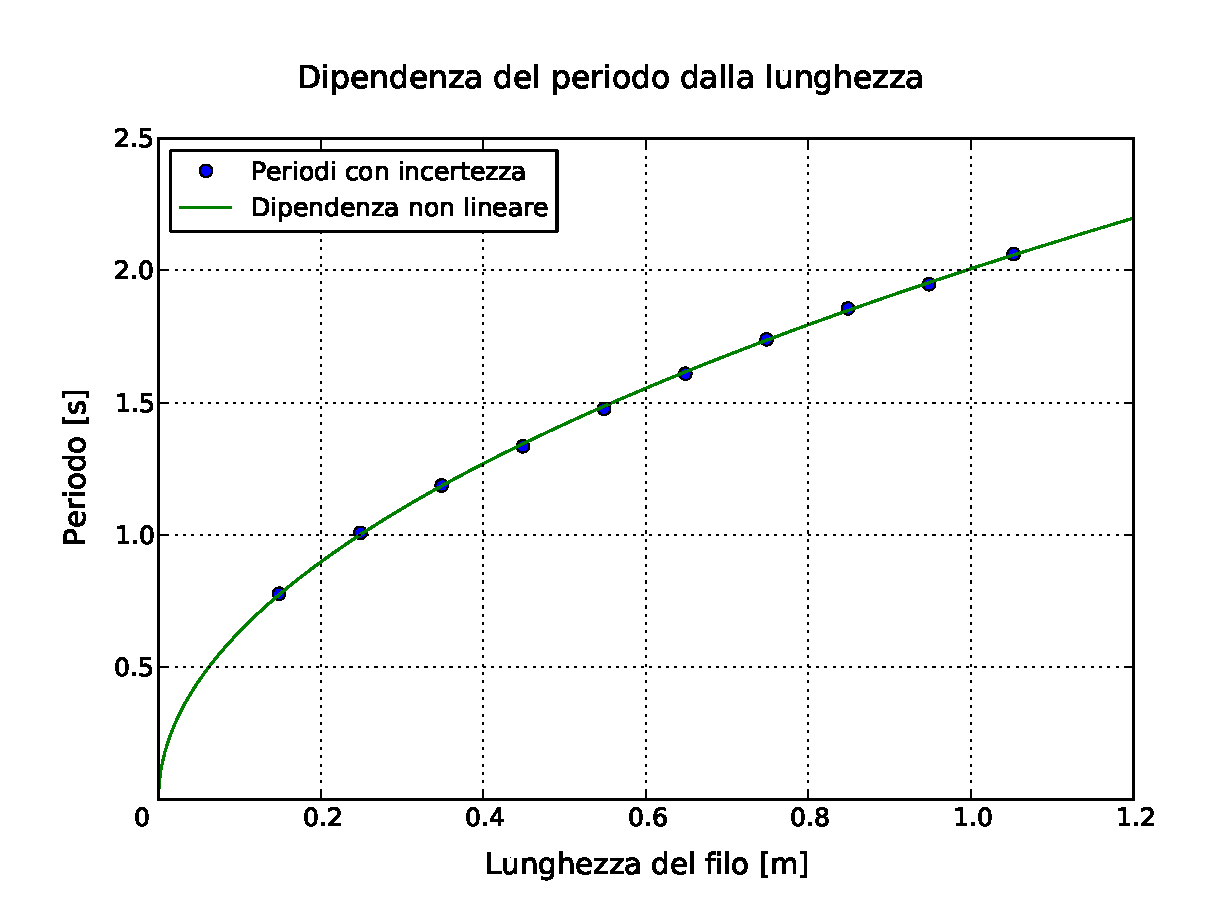
\includegraphics[width=120mm]{immagini/lunghezza_periodo.pdf}
    \caption{Il grafico in figura mostra il periodo del pendolo in funzione della lunghezza del filo.
        Le barre di errore non sono mostrate in quanto sono dell'ordine di grandezza dei punti. Si
        nota immediatamente l'andamento non lineare dei dati sperimentali. La curva in
        figura è la funzione $\mathcal{T} = a\ell^b$ con i valori di $a$ e $b$ calcolati con la regressione
        nel paragrafo \ref{l_regressione}.}
    \label{fig:lunghezza_periodo}
\end{SCfigure}

\begin{SCfigure}[][p]
    \centering
    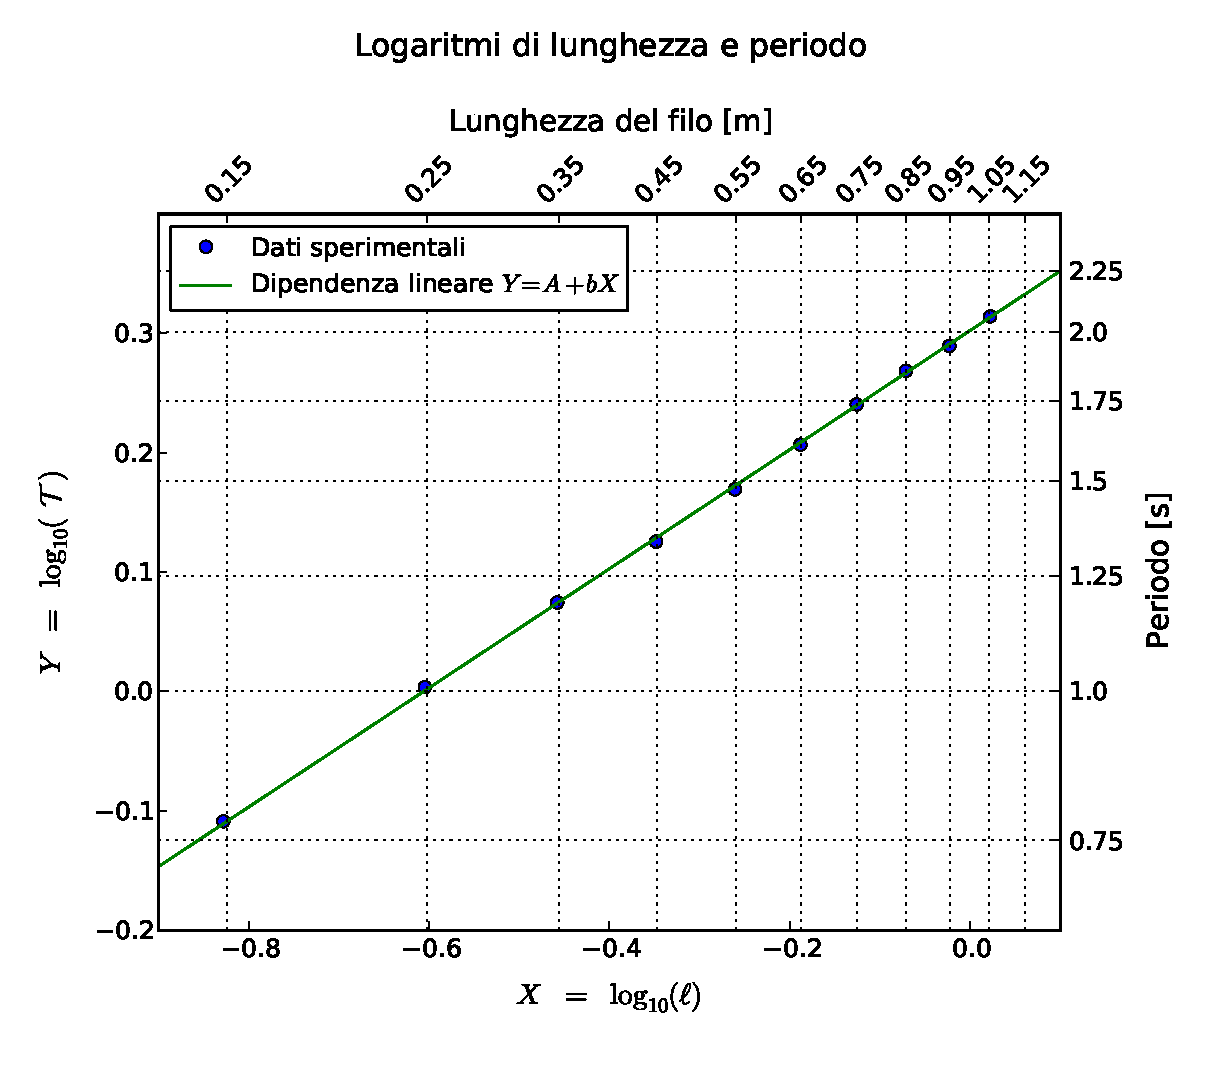
\includegraphics[width=120mm]{immagini/log.pdf}
    \caption{Il grafico è analogo a quello nella figura \ref{fig:lunghezza_periodo}, con la sola differenza
        che in questo caso si tratta di un plot $X = \log_{10} (\ell)$ versus $Y = \log_{10} (\mathcal{T})$, o, equivamentemente,
        gli assi sono in scala logaritmica. Le barre d'errore non sono mostrate poiché invisibili a questa scala.
        In questo grafico si nota la relazione lineare tra $X$ e $Y$, rappresentata dalla retta $Y = A + bX$, con $A$ e $b$ calcolati
    mediante regressione. Notare che $X$ e $Y$ sono numeri puri poichè si fa il logaritmo dei soli valori numerici di $\ell$ e $\mathcal{T}$.}
    \label{fig:lunghezza_periodo_log}
\end{SCfigure}

\label{l_pred_teo}

Graficando i dati ottenuti nel paragrafo precedente, ci si accorge immediatamente (si veda
la figura \ref{fig:lunghezza_periodo}) che il periodo del pendolo dipende dalla lunghezza
del suo filo, come correttamente previsto dalla teoria. Tuttavia la dipendenza è chiaramente non lineare.

Dall'espressione (\ref{eq:periodo_pendolo}) per il periodo del pendolo semplice, si sa che
il periodo vale

\begin{equation}
    \mathcal{T} = 2\pi\sqrt{\frac{\ell}{g}}
    \tag{\ref{eq:periodo_pendolo}}
\end{equation}

Tuttavia qui assumiamo come ipotesi una dipendenza del tipo:

\begin{equation}
    \mathcal{T} = a\ell^b
    \label{eq:ipotesi}
\end{equation}
%
dove $a$ e $b$ sono due costanti\footnote{$b$ è adimensionale, mentre $a$ deve avere dimensioni [$\text{s}\,\text{m}^{-b}$] affinché le unità di misura l'equazione (\ref{eq:ipotesi}) siano corrette}.
Dal grafico in figura \ref{fig:lunghezza_periodo} si può intuire una dipendenza di questo genere.
Confrontando l'equazione (\ref{eq:periodo_pendolo}) con la (\ref{eq:ipotesi}) otteniamo che, secondo il modello
del pendolo semplice, deve valere

\begin{equation}
    a = \frac{2\pi}{\sqrt{g}} \; \frac{\text{s}}{\sqrt{\text{m}}} = 2.006 \qquad \qquad b = \frac{1}{2}
\end{equation}
%
dove per il calcolo di $a$ abbiamo utilizzato il valore $g = \SI{9.806}{\meter\per\square\second}$, di cui trascuriamo l'incertezza.

Queste sono le predizioni teoriche del modello del pendolo semplice. Calcolando $a$ e $b$ dai dati sperimentali
possiamo quindi verificare la correttezza della formula (\ref{eq:periodo_pendolo}).

Vogliamo ora linearizzare l'equazione (\ref{eq:ipotesi}) per poter utilizzare la regressione lineare e ricavare $a$ e $b$.
Al tal fine, definiamo due nuove variabili\footnote{Da notare che $X$ e $Y$, e di conseguenza le loro incertezze,
sono grandezze adimensionali poiché
le funzioni trascendenti, come il logaritmo, hanno argomenti e valori adimensionali. Nella relazione viene sottinteso
che i valori $\ell$ e $\mathcal{T}$, quando sono argomento di logaritmi, indicano solo il valore numerico e non la grandezza fisica
\emph{lunghezza del filo} o \emph{periodo del pendolo}.}:

\begin{equation}
    X := \log_{10}{(\ell)} \qquad \qquad Y := \log_{10}{(\mathcal{T})}
    \label{eq:vars}
\end{equation}

Le incertezze su $X$ e $Y$, calcolate con la regola di propagazione, sono

\begin{equation}
    \delta X = \frac{\log_{10}(e)}{\ell}\delta \ell
    \qquad \qquad
    \delta Y = \frac{\log_{10}(e)}{\mathcal{T}}\delta\mathcal{T}
    \label{eq:delta_XY}
\end{equation}

Quindi, applicando ad entrambi i membri della (\ref{eq:ipotesi}) il logaritmo, si ottiene\footnote{
Anche $A$ è adimensionale.}

\begin{equation}
    Y = \log_{10} (\mathcal{T}) = \log_{10} (a) + b \log_{10} (\ell) = A + b X
\end{equation}
%
dove $A := \log_{10} a$ e dunque $a = 10^A$. La legge trovata è lineare, come mostrato dal grafico
in Figura \ref{fig:lunghezza_periodo_log}, e si può quindi utilizzare la consueta procedura di fit.

%\begin{table}
%    \centering
%    \begin{tabular}{c c c c}
%    \end{tabular}
%\end{table}

\subsubsection{Regressione}
\label{l_regressione}

Per cominciare abbiamo calcolato, per ogni coppia ($\ell_i$, $\mathcal{T}_i$), i valori $X_i$ e $Y_i$
e le relative incertezze $\delta X_i$ e $\delta Y_i$, usando le formule (\ref{eq:vars}) e (\ref{eq:delta_XY}).

Procediamo ora con il calcolo dei parametri A e b tramite regressione lineare. 
La regressione si basa sulla minimizzazione della funzione

\begin{equation}
    \sum_{i=1}^N \frac{(Y_i - A - bX_i)^2}{(\delta Y_i^{\text{tot}})^2}
    \qquad \qquad \text{dove} \quad
    \delta Y_i^{\text{tot}} = \sqrt{\delta Y_i^2 + b^2 \delta X_i^2}
    \label{eq:min_quad}
\end{equation}

Questa funzione misura la discrepanza tra legge lineare e dati sperimentali. Minimizzando la (\ref{eq:min_quad}) si ottengono
i valori di $A$ e $b$, ovvero la retta, che interpretano in modo ``migliore'' i dati.

Come prima cosa si è stimato il parametro b per trasferire l'incertezza dalle X alle Y.
La stima è stata ottenuta ignorando l'incertezza sulle X, ovvero ponendo $\delta Y_i^{\text{tot}} = \delta Y_i$ e facendo un fit preliminare.
Dai calcoli risulta:

\begin{equation}
    b' + \delta b' = 0.499 \pm 0.002
\end{equation}

Abbiamo utilizzato questo valore $b'$ per trasferire l'incertezza e calcolare $\delta Y_i^{\text{tot}}$. Minimizzando nuovamente la 
(\ref{eq:min_quad}) con i nuovi valori dell'incertezza trovati, si ha che:

\begin{equation}
    A = 0.3024 \qquad \qquad b = 0.499
\end{equation}

Le incertezze su $A$ e $b$ si possono ricavare con la propagazione dell'incertezza e valgono:

\begin{equation}
    \delta A = 0.0005 \qquad \qquad \delta b = 0.002
\end{equation}

Prima di proseguire notiamo che il valore di $b$ ricavato dalla regressione è compatibile con la stima $b'$
ricavata dal fit preliminare, in quanto i risultati sono uguali entro l'incertezza. Questo indica anche che
l'incertezza trasferita dalle $X$ è trascurabile rispetto all'incertezza sulle $Y$.

	\subsection{Conclusioni intermedie !-!-!-!-!-!-!-!-!-!-!-!-!-!-!}
	---

\newpage
\section{Misurazione dell'accelerazione di gravità}
%\input{misurazione.tex}
Nell'approssimazione di piccole oscillazioni, si può sfruttare la relazione che legal'accelerazione di gravità $g$ e la lunghezza $\ell$ del pendolo semplice al periodo $\mathcal{T}$ dello stesso, per ricavare l'accelerazione di gravità:
\begin{equation}
	g \,\, = \,\, (2 \pi / \mathcal{T})^2 \ell
\end{equation}
	\subsection{Analisi tabella}
	---

	\subsection{Determinare l'accelerazione di gravità dalla tabella}
	---

	\subsection{Determinare l'accelerazione di gravità dal grafico}
	Al punto $\bigotimes$ la relazione tra periodo del pendolo e lunghezza era stata espressa nella formula
\begin{equation*}
	\mathcal{T} \,\, = \,\, ab^{\ell}
\end{equation*}
che confrontata con l'equazione $\bigotimes$ \ref{equazione del pendolo} permette di ricavare $a \,\, = \,\, 2 \pi / \sqrt{g}$, da cui si ottiene:
\begin{equation}
	g \,\, = \,\, \left( \frac{2 \pi}{a}\right)^2 \quad\quad e \quad\quad \delta g \,\, = \,\, \frac{\vert dg \vert}{\vert da\vert} \delta a = \frac{8 \pi^2}{a^3} \delta a
\end{equation}

Quindi si ricava il valore:
\begin{equation}
	g \pm \delta g \,\, = \,\, \ast\ast,\ast \pm \ast,\ast \,\, ms^{-2}
\end{equation}
	\subsection{Test del chi quadro}
	---

	\subsection{Confronto con valore tabulati}
	---


\newpage
\section{Conclusioni}
\section{Conclusioni}
In questo esperimento abbiamo utilizzato due diversi procedimenti meccanici per la misura di una stessa grandezza: la costante elastica della molla. I due procedimenti si differenziano per il diverso utilizzo della molla: il primo necessita di un uso statico (misurazione dell'elongazione), mentre il secondo di un uso dinamico (misurazione del periodo di oscillazione). Ogni procedimento ha portato all'ottenimento di un valore della costante elastica e, inoltre, ogni valore della costante è stato a sua volta ottenuto sia con procedure grafiche sia con procedure analitiche.
Seguire non una sola procedura, ma entrambe, ci ha permesso una maggiore sicurezza sulla validità del risultato ottenuto. Ogni procedura ha infatti funto da controprova per l'altra e, come mostrato nel precedente paragrafo, i coefficienti elastici ricavati con il metodo statico e con il metodo dinamico risultano compatibili, ponendo come fattore di copertura $k\,=\,3$.

In questo stesso esperimento ci interessava, inoltre, verificare la linearità della risposta della molla in funzione della forza ad essa applicata. Questo obiettivo è stato raggiunto e, come si può vedere dalle tabelle e dai grafici, la linearità è stata appurata in un adeguato range di valori.
È in aggiunta stato verificato che la molla non si deformasse in modo definitivo a causa dei pesi a cui era stata sottoposta, vanificando tutto l'esperimento.
\\
\\


\textbf{Disclaimer}: Nonostante i componenti del gruppo B11 ci vogliano affibbiare la colpa del fatto che il loro esperimento non è andato a buon fine, noi decliniamo apertamente ed a gran voce ogni responsabilità.

\end{document}
